% -*- latex -*-
%%%%%%%%%%%%%%%%%%%%%%%%%%%%%%%%%%%%%%%%%%%%%%%%%%%%%%%%%%%%%%%%
%%%%%%%%%%%%%%%%%%%%%%%%%%%%%%%%%%%%%%%%%%%%%%%%%%%%%%%%%%%%%%%%
%%%%
%%%% This text file is part of the source of 
%%%% `Parallel Programming in MPI and OpenMP'
%%%% by Victor Eijkhout, copyright 2012-6
%%%%
%%%% mpi-started.tex : introductory chapter about MPI
%%%%
%%%%%%%%%%%%%%%%%%%%%%%%%%%%%%%%%%%%%%%%%%%%%%%%%%%%%%%%%%%%%%%%
%%%%%%%%%%%%%%%%%%%%%%%%%%%%%%%%%%%%%%%%%%%%%%%%%%%%%%%%%%%%%%%%

In this chapter you will learn the use of the main tool for 
distributed memory programming: the \acf{MPI} library.
The \ac{MPI} library has about 250 routines, many of which you may
never need. Since this is a textbook, not a reference manual, we will
focus on the important concepts and give the important routines for
each concept. What you learn here should be enough for most common
purposes. You are advised to keep a reference document handy, in
case there is a specialized routine, or to look up subtleties about
the routines you use.

\Level 0 {Distributed memory and message passing}

In its simplest form, a distributed memory machine is a collection of
single computers hooked up with network cables. In fact, this has a name:
a \indexterm{Beowulf cluster}. As you recognize from that setup, 
each processor can run an independent program, and has its own memory
without direct access to other processors' memory. MPI is the magic
that makes multiple instantiations of the same executable run
so that they know about each other and can exchange data through the 
network.

One of the reasons that MPI is so successful as a tool for high
performance on clusters is that it is very explicit: the programmer
controls many details of the data motion between the processors.
Consequently, a capable programmer can write very efficient code with MPI.
Unfortunately, that programmer will have to spell things out
in considerable detail. For this reason, people sometimes call MPI
`the assembly language of parallel programming'. If that sounds scary,
be assured that things are not that bad. You can get started 
fairly quickly with MPI, using just the basics,
and coming to the more sophisticated tools 
only when necessary.

Another reason that MPI was a big hit with programmers is that
it does not ask you to learn a new language: it is a library that 
can be interface to C/C++ or Fortran; there are even bindings to Python.
A~related point is that it is easy to install: there are free implementations
that you can download and install on any computer that has a Unix-like
operating system, even if that is not a parallel machine.

\Level 0 {History}

Before the MPI standard was developed in 1993-4, there were many
libraries for distributed memory computing, often proprietary
to a vendor platform. MPI standardized the inter-process communication
mechanisms. Other features, such as process management in \indexterm{PVM},
or parallel I/O were omitted. Later versions of the standard
have included many of these features.

Since MPI was designed by a large number of academic and commercial
participants, it quickly became a standard. A~few packages
from the pre-MPI era, such as \indexterm{Charmpp}~\cite{charmpp},
are still in use since they support mechanisms that do not exist
in MPI.

\Level 0 {Basic model}
\label{sec:mpiexec}

Here we sketch the two most common scenarios for using MPI. In the
first, the user is working on an interactive machine, which has
network access to a number of hosts, typically a network of workstations;
see figure~\ref{fig:mpi-interactive}.
\begin{figure}[ht]
  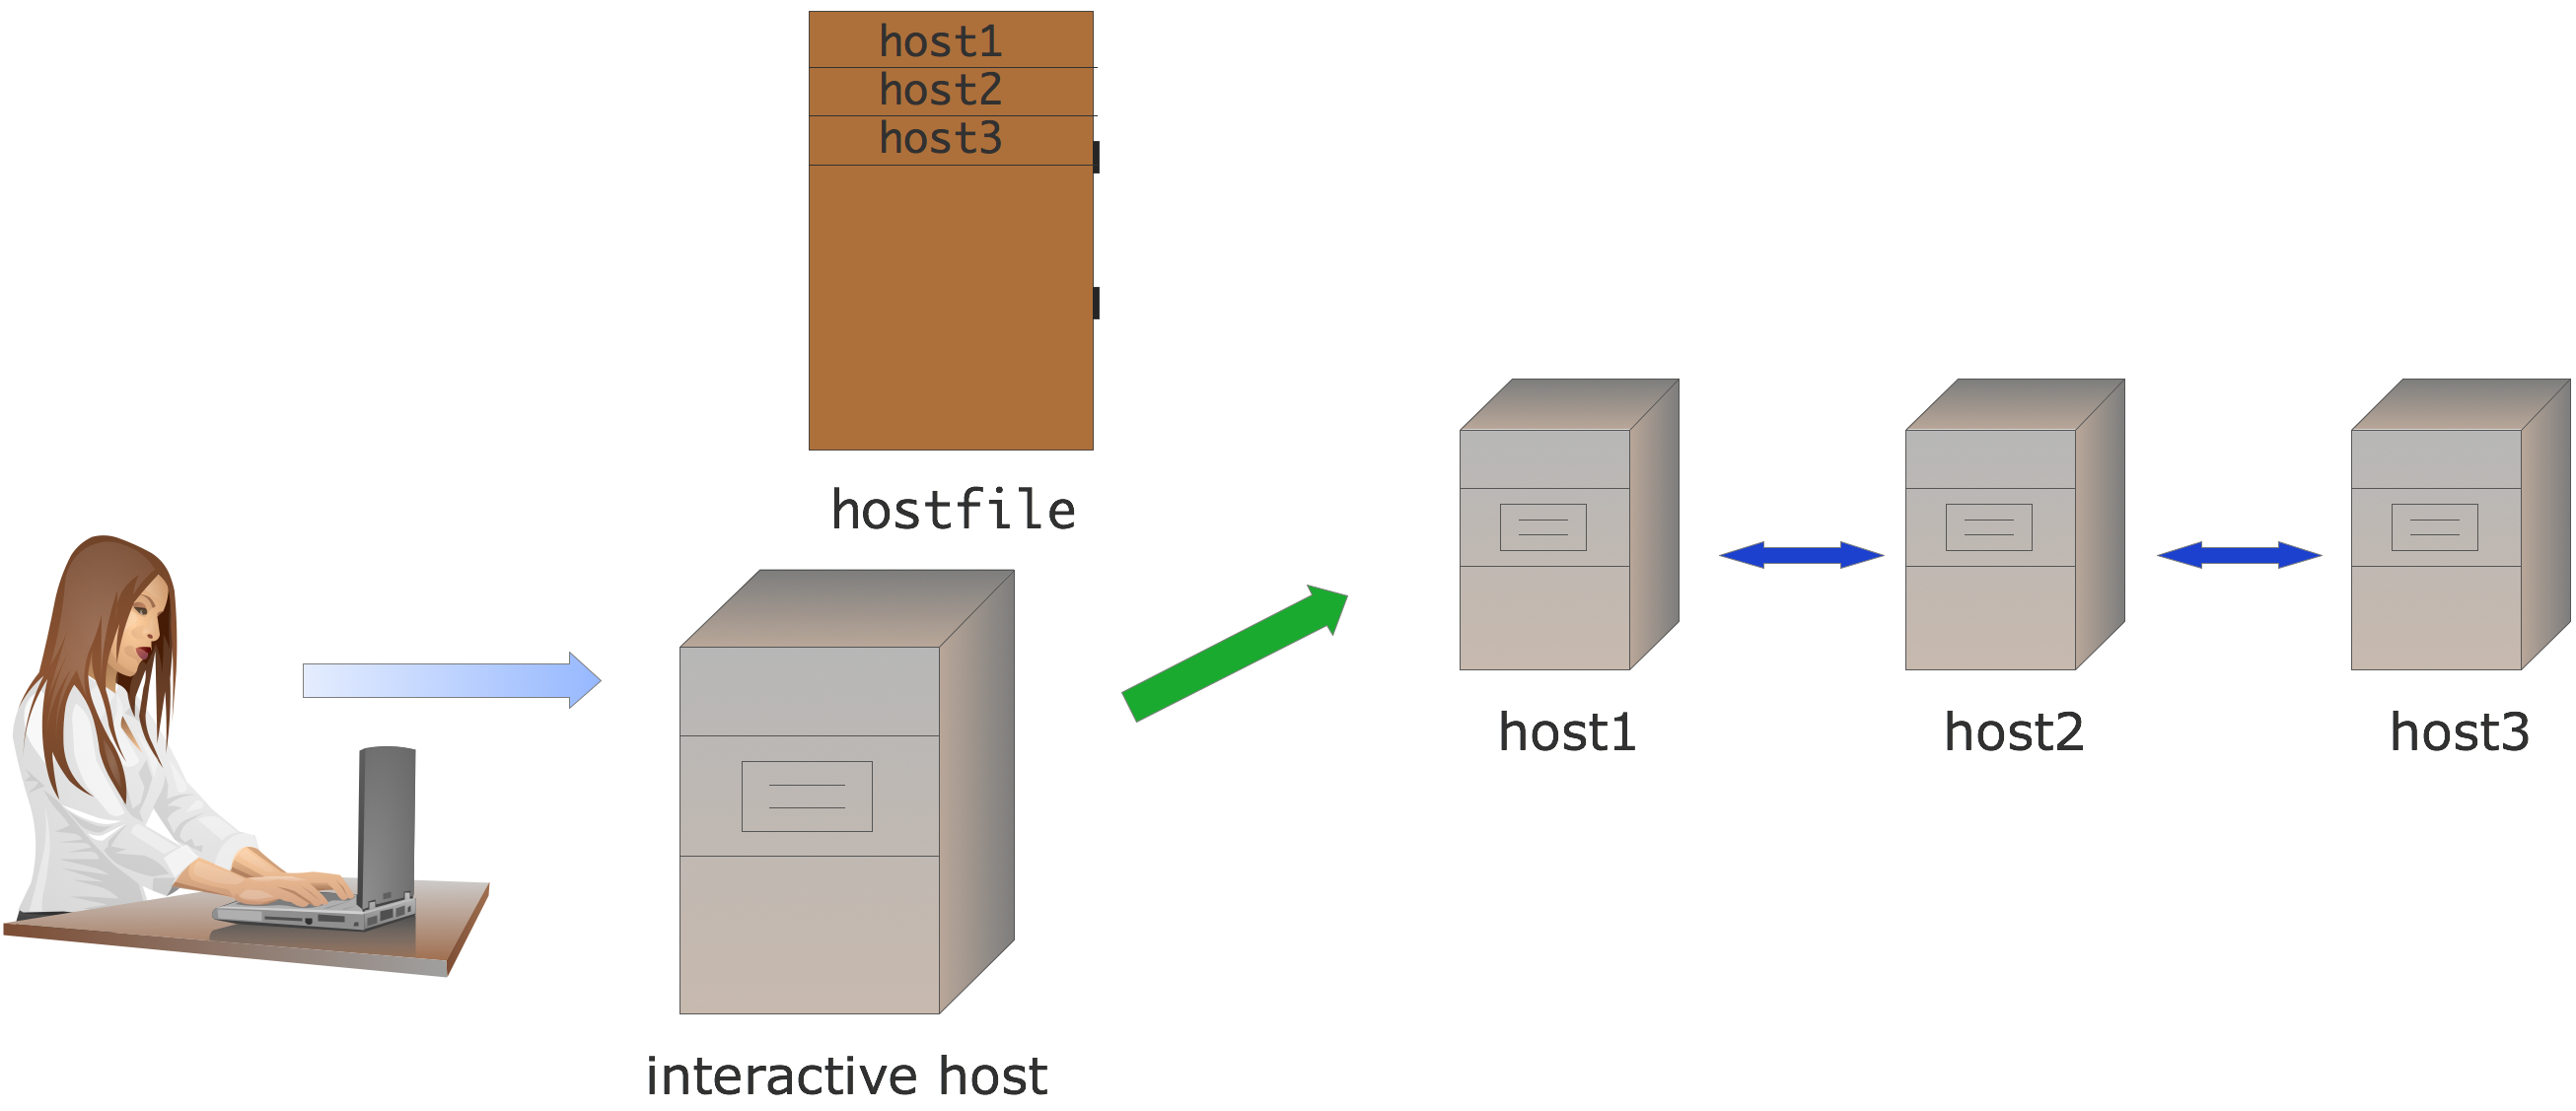
\includegraphics[scale=.12]{graphics/mpi-interactive}
  \caption{Interactive MPI setup}
  \label{fig:mpi-interactive}
\end{figure}
The user types the command \n{mpiexec}\index{mpiexec}\footnote
{A command variant is \texttt{mpirun}\index{mpirun}; your local cluster
  may have a different mechanism.}
and supplies
\begin{itemize}
\item The number of hosts involved,
\item their names, possibly in a hostfile,
\item and other parameters, such as whether to include the interactive
  host; followed by
\item the name of the program and its parameters.
\end{itemize}
The \n{mpirun} program then makes an \n{ssh}\index{ssh} connection
to each of the hosts, giving them sufficient information that they 
can find each other. All the output of the processors is piped through the 
\n{mpirun} program, and appears on the interactive console.

In the second scenario (figure~\ref{fig:mpi-batch}) the user prepares
a \indextermbus{batch}{job} script with commands, and these will be
run when the \indextermbus{batch}{scheduler} gives a number of hosts
to the job.
\begin{figure}[ht]
  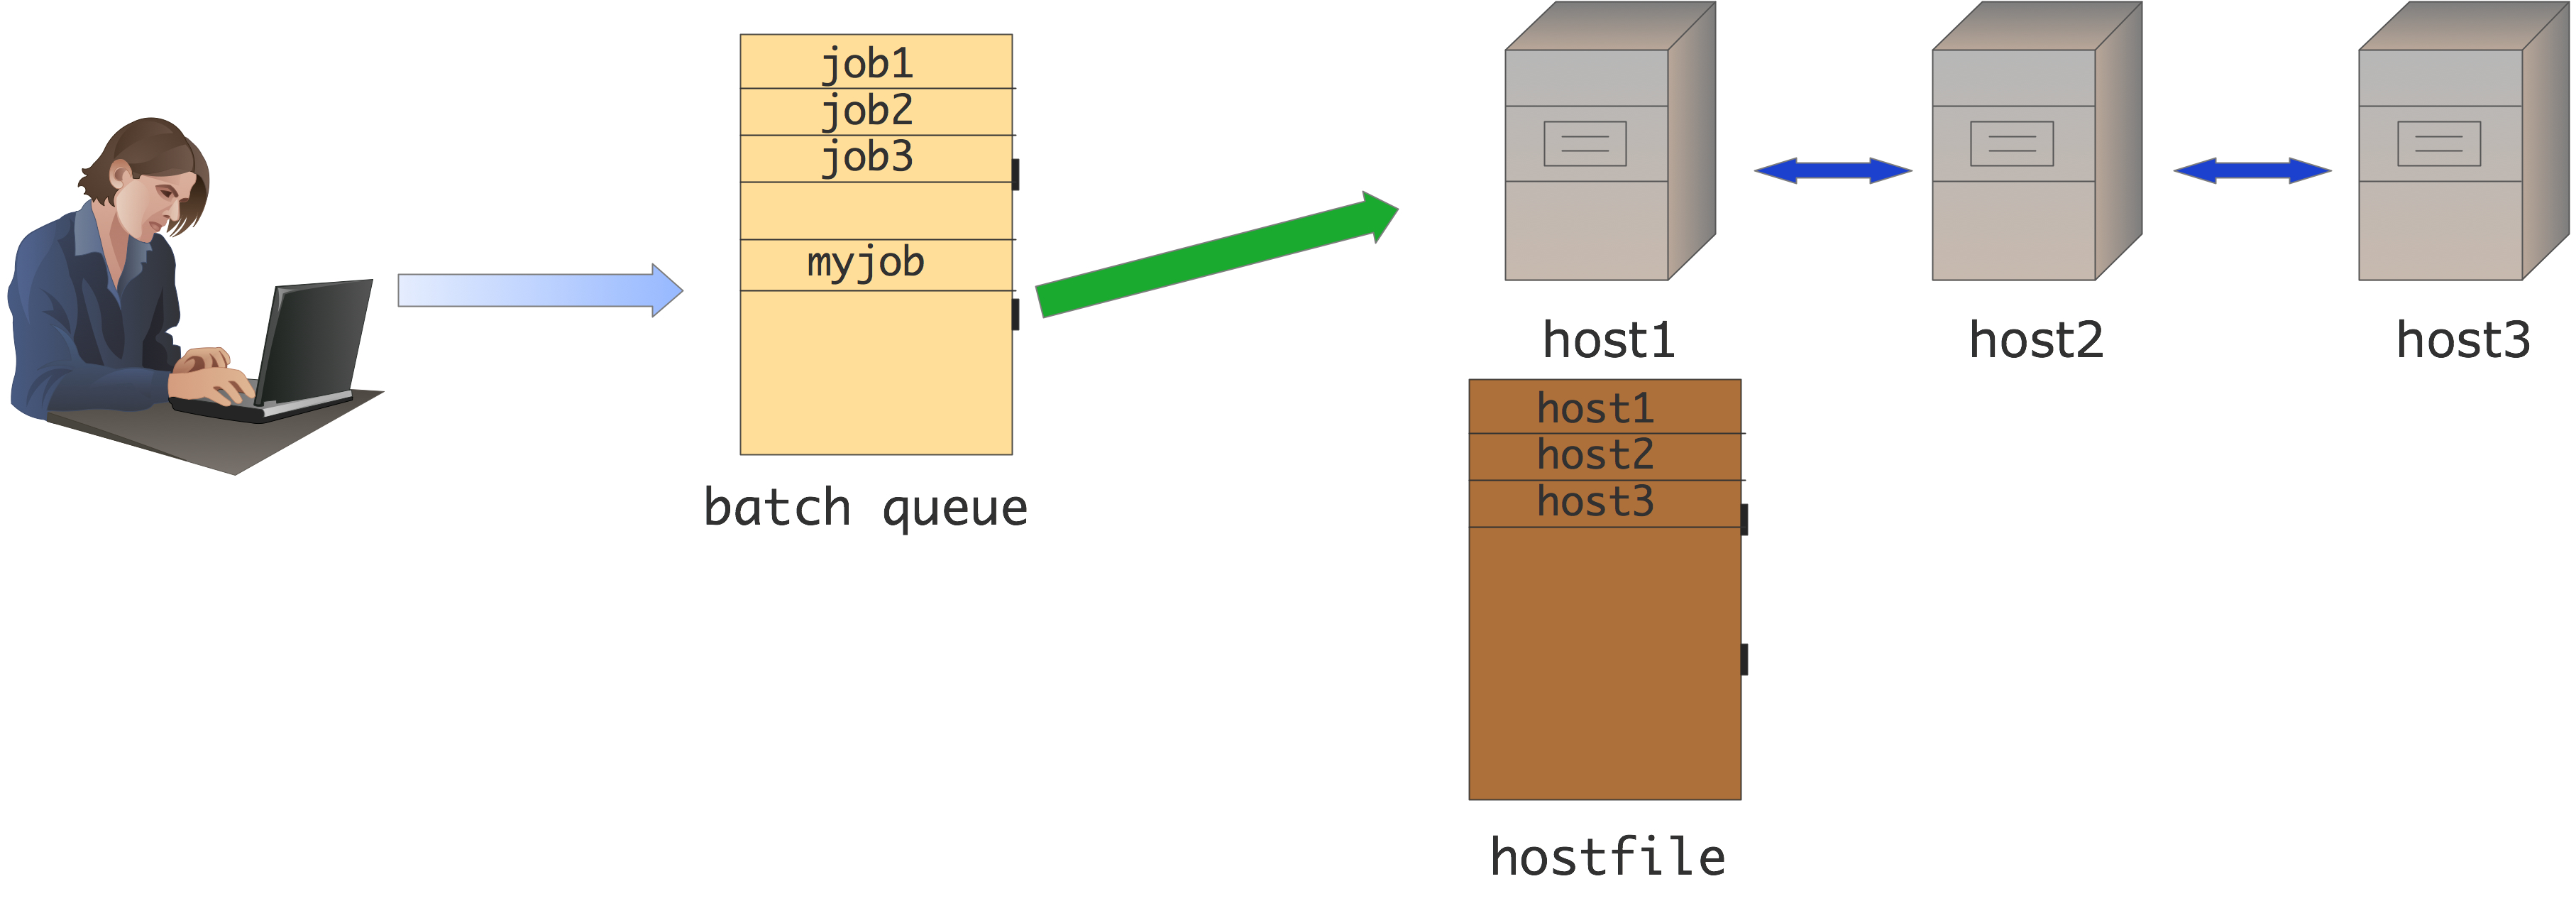
\includegraphics[scale=.1]{graphics/mpi-batch}
  \caption{Batch MPI setup}
  \label{fig:mpi-batch}
\end{figure}
Now the batch script contains the \n{mpirun} command%
\begin{istc}
, or some variant such as \n{ibrun}\index{ibrun}%
\end{istc}
, and the hostfile is dynamically generated when the job starts.
Since the job now runs at a time when the user may not be logged in, 
any screen output goes into an output file.

You see that in both scenarios the parallel program is started
by the \n{mpirun} command using
an \ac{SPMD} mode of execution: all hosts execute the same program.
It is possible for different hosts to execute different programs,
but we will not consider that in this book.

\Level 0 {Making and running an MPI program}

MPI is a library, called from programs in ordinary programming languages
such as C/C++ or Fortran. To compile such a program you use your regular
compiler:
\begin{verbatim}
gcc -c my_mpi_prog.c -I/path/to/mpi.h
gcc -o my_mpi_prog my_mpi_prog.o -L/path/to/mpi -lmpich
\end{verbatim}
However, MPI libraries may have different names between different
architectures, making it hard to have a portable makefile. Therefore,
MPI typically has shell scripts around your compiler call:
\begin{verbatim}
mpicc -c my_mpi_prog.c
mpicc -o my_mpi_prog my_mpi_prog.o
\end{verbatim}

MPI programs can be run on many different architectures. Obviously it
is your ambition (or at least your dream) to run your code on a
cluster with a hundred thousand processors and a fast network. But
maybe you only have a small cluster with
plain \indexterm{ethernet}. Or maybe you're sitting in a plane, with
just your laptop. An MPI program can be run in all these
circumstances~--~within the limits of your available memory of course.

The way this works is that you do not start your executable directly,
but you use a program, typically called \n{mpirun}\index{mpirun} or
something similar, which makes a connection to all available
processors and starts a run of your executable there. So if you have a
thousand nodes in your cluster, \n{mpirun} can start your program once
on each, and if you only have your laptop it can start a few instances
there. In the latter case you will of course not get great
performance, but at least you can test your code for correctness.

\begin{tacc}
  \begin{pythonnote}
    Load the TACC-provided python:
\begin{verbatim}
module load python
\end{verbatim}
and run it as:
\begin{verbatim}
ibrun python-mpi yourprogram.py
\end{verbatim}
  \end{pythonnote}
\end{tacc}

\Level 0 {Language bindings}

\Level 1 {C/C++}
\index{C!MPI bindigs|see{MPI, C/C++ bindings}}
\index{C++!MPI bindigs|see{MPI, C/C++ bindings}}
\index{MPI!C/C++ bindings|(}

The MPI library is written in~C. Thus, its bindings are the most natural
for that language.

C++ bindings existed at one point, but they were declared deprecated,
and have been officially removed in the \emph{MPI~3}%
\index{MPI!3!C++ bindings removed}
The \indexterm{boost} library has its own version of MPI, but it seems
not to be under further development.  A~recent
effort at idiomatic C++ support is \indexterm{MPL}
\url{http://numbercrunch.de/blog/2015/08/mpl-a-message-passing-library/}.

\index{MPI!C/C++ bindings|)}

\Level 1 {Fortran}
\index{Fortran!MPI bindings|see{MPI, Fortran bindings}}
\index{Fortran2008!MPI bindings|see{MPI, Fortran2008 bindings}}
\index{MPI!Fortran bindings|(}

The \emph{Fortran bindings} for MPI look very much like the C~ones, except that
each routine has a final \indexterm{error return} parameter.

\begin{fortrannote}
  Other Fortran-specific differences will be indicated with a note
  like this.
\end{fortrannote}

\index{MPI!Fortran2008 bindings|(}
%
In the \emph{MPI~3}%
\index{MPI!3!Fortran2008 interface} standard,
an MPI implementation providing a Fortran interface must provide a
module named \n{mpi_f08} that can be used in a Fortran program.
This defines MPI functions that return an integer result, rather than
having a final parameter. It also defines proper interfaces, making
type checking possible. For details see \url{http://mpi-forum.org/docs/mpi-3.1/mpi31-report/node409.htm}.
%
\index{MPI!Fortran2008 bindings|)}

\index{MPI!Fortran bindings|)}

\Level 1 {Python}
\label{sec:python-bind}
\index{Python!MPI bindigs|see{MPI, Python bindings}}
\index{MPI!Python bindings|(}

The \indextermtt{mpi4py} package of \emph{python bindings}
is not defined by the MPI
standards committee. Instead, it is the work of an individual,
\indextermsub{Lisandro}{Dalcin}.

Notable about the Python bindings is that many communication routines
exist in two variants:
\begin{itemize}
\item a version that can send native Python objects. These routines
  have lowercase names such as \n{bcast}; and
\item a version that sends \indexterm{numpy} objects; these routines
  have names such as \n{Bcast}. Their syntax can be slightly different.
\end{itemize}
The first version looks more `pythonic', is easier to write,
and can do things like sending python objects,
but it is also decidedly less efficient since data is packed
and unpacked with \n{pickle}. As a common sense guideline,
use the \n{numpy} interface in the performance-critical parts
of your code, and the native interface only for complicated
actions in a setup phase.

Codes with \texttt{mpi4py} can be interfaced to other languages
through Swig or conversion routines.

Data in \texttt{numpy} can be specified as a simple object,
or \texttt{[data, (count,displ), datatype]}.

\index{MPI!Python bindings|)}

\Level 1 {How to read routine prototypes}
\label{sec:protos}

Throughout the MPI part of this book we will give the reference syntax
of the routines. This typically comprises:
\begin{itemize}
\item The semantics: routine name and list of parameters and what they
  mean.
\item C synxtax: the routine definition as it appears in the
  \indextermtt{mpi.h} file.
\item Fortran syntax: routine definition with parameters, giving
  in/out specification.
\item Python syntax: routine name, indicating to what class it
  applies, and parameter, indicating which ones are optional.
\end{itemize}

These `routine prototypes' look like code but they are not! Here is
how you translate them.

\Level 2 {C}

The typically C routine specification in MPI looks like:
\begin{verbatim}
int MPI_Comm_size(MPI_Comm comm,int *nprocs)
\end{verbatim}
This means that
\begin{itemize}
\item The routine returns an \n{int} parameter. Strictly speaking you
  would use the routine as
\begin{verbatim}
MPI_Comm comm = MPI_COMM_WORLD;
int nprocs;
int errorcode;
errorcode = MPI_Comm_world( MPI_COMM_WORLD,&nprocs
if (errorcode!=0) {
  printf("Routine MPI_Comm_world failed! code=%d\n",errorcode);
  return 1;
}
\end{verbatim}
  However, the error codes are hardly ever useful, and there is not
  much your program can do to recover from an error. Most people call
  the routine as
\begin{verbatim}
MPI_Comm_world( /* parameter ... */ );
\end{verbatim}
\item The first argument is of type \n{MPI_Comm}. This is not a C
  built-in datatype, but it behaves like one. There are many of these
  \n{MPI_something} datatypes in MPI. So you can write:
\begin{verbatim}
MPI_Comm my_comm = MPI_COMM_WORLD; // using a predefined value
MPI_Comm_size( comm, /* remaining parameters */ );
\end{verbatim}
\item Finally, there is a `star' parameter. This means that the
  routine wants an address, rather than a value. You would typically write:
\begin{verbatim}
MPI_Comm my_comm = MPI_COMM_WORLD; // using a predefined value
int nprocs;
MPI_Comm_size( comm, &nprocs );
\end{verbatim}
  Seeing a `star' parameter usually means either: the routine has an
  array argument, or: the routine internally sets the value of a
  variable. The latter is the case here.
\end{itemize}

\Level 2 {Fortran}

The Fortran specification looks like:
\begin{verbatim}
MPI_Comm_size(comm, size, ierror)
INTEGER, INTENT(IN) :: comm
INTEGER, INTENT(OUT) :: size
INTEGER, OPTIONAL, INTENT(OUT) :: ierror
\end{verbatim}
The syntax of using this routine is close to this specification: you
write
\begin{verbatim}
integer :: comm = MPI_COMM_WORLD
integer :: size
CALL MPI_Comm_size( comm, size, ierr )
\end{verbatim}
\begin{itemize}
\item Most Fortran routines have the same parameters as the
  corresponding C routine, except that they all have the error code as
  final parameter, instead of as a function result. As with~C, you can
  ignore the value of that parameter. Just don't forget it.
\item The types of the parameters are given in the specification.
\item Where C routines have \n{MPI_Comm} and \n{MPI_Request} and such
  parameters, Fortran has \n{INTEGER} parameters, or sometimes arrays
  of integers.
\end{itemize}

\Level 3 {Python}

The Python interface to MPI uses classes and objects. Thus, a
specification like:
\begin{verbatim}
MPI.Comm.Send(self, buf, int dest, int tag=0)
\end{verbatim}
should be parsed as follows.
\begin{itemize}
\item First of all, you need the \n{MPI} class:
\begin{verbatim}
from mpi4py import MPI
\end{verbatim}
\item Next, you need a \n{Comm} object. Often you will use the
  predefined communicator
\begin{verbatim}
comm = MPI.COMM_WORLD
\end{verbatim}
\item The keyword \n{self} indicates that the actual routine \n{Send}
  is a method of the \n{Comm} object, so you call:
\begin{verbatim}
comm.Send( .... )
\end{verbatim}
\item Parameters that are listed by themselves, such as \n{buf}, as
  positional. Parameters that are listed with a type, such as \n{int
    dest} are keyword parameters. Keyword parameters that have a value
  specified, such as \n{int tag=0} are optional, with the default
  value indicated. Thus, the typicall call for this routine is:
\begin{verbatim}
comm.Send(sendbuf,dest=other)
\end{verbatim}
  specifying the send buffer as positional parameter, the destination
  as keyword parameter, and using the default value for the optional tag.
\end{itemize}
Some python routines are `class methods', and their specification
lacks the \n{self} keyword. For instance:
\begin{verbatim}
MPI.Request.Waitall(type cls, requests, statuses=None)
\end{verbatim}
would be used as
\begin{verbatim}
MPI.Request.Waitall(requests)
\end{verbatim}
